\subsection{Одноточечное скрещивание}\label{SetOfOperatorsAlgorithms:SinglepointCrossover}

Идентификатор: \textbf{SinglepointCrossover}.

Данный оператор скрещивания используется для бинарных векторов.

Пусть имеется два родителя (родительские хромосомы) $ \overline{Parent}^1 $ и $ \overline{Parent}^2$. В случайном месте происходит разрыв между двумя позициями генов в обеих хромосомах. После этого хромосомы обмениваются частями, в результате чего образуются два потомка. Из них выбирается случайно один потомок, который и передается в качестве результата оператора скрещивания. То есть скрещивание происходит по формулам:

\begin{align}
\label{SetOfOperatorsAlgorithms:eq:SinglepointCrossover}
&Crossover \left( \overline{Parent}^1, \overline{Parent}^2, DataOfCros\right)=Random \left(\left\lbrace \overline{Offspring}^1; \overline{Offspring}^2\right\rbrace  \right), \\
&R=Random\left( \left\lbrace 2; 3; \ldots; n\right\rbrace \right); \nonumber \\
& \overline{Offspring}^1_i=\overline{Parent}^1_i, i=\overline{1,R-1};\nonumber\\
&  \overline{Offspring}^1_i=\overline{Parent}^2_i, i=\overline{R,n};\nonumber\\
&\overline{Offspring}^2_i=\overline{Parent}^2_i, i=\overline{1,R-1};\nonumber\\
& \overline{Offspring}^2_i=\overline{Parent}^1_i, i=\overline{R,n};\nonumber\\
&\overline{Offspring}^1\in X, \overline{Offspring}^2\in X.\nonumber
\end{align}

\textbf{Пример.} Для всех видов скрещивания будем использовать двух родителей: $\overline{Parent}^1\hmm={\left( 0; 1; 0; 1; 1; 1; 0; 0\right)}^\mathrm{T}  $ и $\overline{Parent}^2={\left( 1; 1; 0; 0; 1; 0; 1\right)}^\mathrm{T}  $. Одноточечное скрещивание показано на рисунке:

\begin{figure} [H] 
  \center
  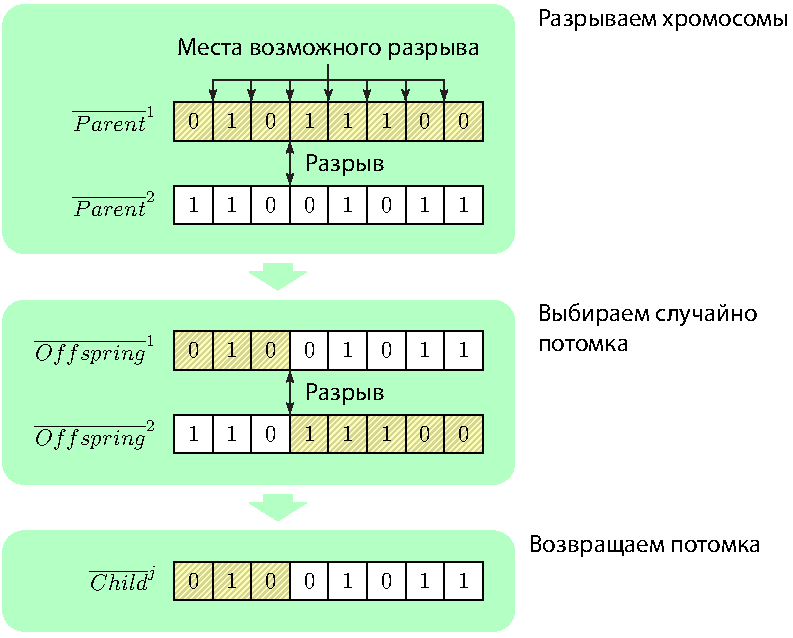
\includegraphics [scale=0.8] {SinglepointCrossover}
  \caption{Механизм работы одноточечного скрещивания} 
  \label{SetOfOperatorsAlgorithms:img:SinglepointCrossover}  
\end{figure}

$ DataOfCros $ не содержит каких-либо параметров относительно данного типа скрещивания.

В библиотеке \textbf{HarrixMathLibrary} данная селекция реализуется через функцию \textbf{TMHL\_SinglepointCrossover}:

\href{https://github.com/Harrix/HarrixMathLibrary}{https://github.com/Harrix/HarrixMathLibrary}